\section{System Design}\label{sec:system-design}

\subsection{Architecture Design}\label{subsec:architecture-design}

\subsubsection{Project Hardware Architecture}

\begin{figure}[htbp]
    \centering
    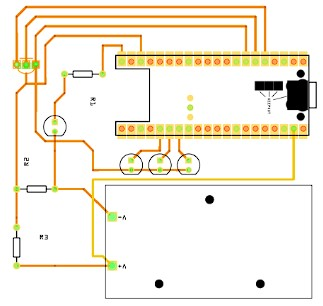
\includegraphics[width=\linewidth]{images/pcbDiagram}
    \caption{PCB Diagram}
    \label{fig:pcbDiagram}
\end{figure}

The PCB (Printed Circuit Board Diagram) diagram depicts the layout of the DIY security
circuit board. %
It shows the placement of components and their interconnections on the board, as well as any necessary information related to the fabrication and assembly of
the board. %
While a circuit diagram provides a schematic representation of the electrical connections between components, the PCB diagram shows the physical layout of the
components and the soldering points between them and the soldering layers. %
It is
important for the efficient routing of traces and connections and will be used during
the fabrication process. %

The PCB will have 3 main components, the Raspberry Pi Pico W Microcontroller with
2.4Ghz Wi-Fi Module which is in the right top corner, the 9V Battery input in the
right bottom corner, and finally, it will have the 5.8Ghz Microwave Motion Sensor
which is in the left top corner of the board. %
The motion sensor emits electromagnetic waves which are then reflected back to the receiver and analyzed. %
If the waves are altered that means the object that reflected them is moving. %
The board also will have 4 LED indicators for showing the WI-FI connection indicator, power indicator,
motion detection indicator, and connection to backend service indicator. %
Rx-Tx serial communication will be used between the microcontroller and motion sensor,
for all other communication GP pins will be used. %

The hardware has two main components, the motion detector, and the microcontroller. %
The microcontroller uses Rx-Tx serial communication to send and receive information
into the motion detector in the form of bits, which can be used to send and receive
instructions. %
Microwave Sensor out signal is used to detect the motion itself. %
As the microcontroller comes with an integrated Wi-Fi module, it will be used to communicate with the backend by sending and receiving API requests.
The device will enter sleep mode and only be activated during motion detection,
this will allow us to lower the power consumption significantly. %
All the hardware will be programmed in C and Micropython. %

The microcontroller has an integrated server with web UI, which allows users
to connect to it with their home devices such as smartphones, and do an easy setup
of the systems, such as the Wi-Fi module. %
UI also provides basic information regarding the status of the motion detection device, battery lifetime, and other necessary
information. %
The microcontroller has full control over the motion detector which allows users to do the precise configuration of system parameters, such as motion
detection range, sensitivity, etc. %

\begin{figure}[htbp]
    \centering
    \includegraphics[width=\linewidth, angle=-90]{images/hardwarearchitecture}
    \caption{Project Hardware Architecture}
    \label{fig:hardwareArchitecture}
\end{figure}


\subsubsection{Project Software Architecture}

The Notification Service is responsible for processing and sending SMS notifications
to users when the motion is detected. %
It receives the motion detection information through requests from sensor management software and sends SMS notifications to the
registered mobile numbers. %
Notification Service will integrate SMS gateway using Twilio API for communication with Client Devices.
A database is required to store information about the user systems, such as user information, sensor information,
and notification settings. %
The Reporting and Analytics component is responsible for generating reports on the system’s performance, such as the number of motion
detections per day and average response time. %
It will help to analyze and further improve the quality of the systems. %

\begin{figure}
    \centering
    \begin{adjustbox}{width=\linewidth}
        \begin{tikzpicture}
            \begin{umlcomponent}[x=4,y=0]{Cloud Workspace}
                \umlbasiccomponent[x=1,y=-2]{User Management Service - UI}
                \umlbasiccomponent[x=1,y=-4.5]{Reporting/Analytics Service}
                \umlbasiccomponent[x=1,y=-6.8]{Database}
                \begin{umlcomponent}[x=5.5,y=-3]{Notification Service}
                    \umlbasiccomponent[x=1, y=-2]{Twilio API}
                \end{umlcomponent}
            \end{umlcomponent}
            \umlbasiccomponent[x=4.5,y=-10.6]{Sensor Management Software}
            \umlbasiccomponent[x=11,y=-10.6]{Client Device}

            \draw[-latex, line width=1.5pt, dashed] (Sensor Management Software.north) -- (Notification Service.west);
            \draw[-latex, line width=1.5pt, dashed] (Twilio API.south) -- (Client Device.north);
        \end{tikzpicture}
    \end{adjustbox}
    \caption{Software Architecture}
    \label{fig:softwareArchitecture}
\end{figure}

User Management Service (UI) will provide an interface for users to register and
authenticate their devices and configure notification settings. %
It will provide an event log, which allows users to manage events related to sensors. %
Additionally, it will have an audit trail of all activity in the system, including user activity. %
The systems above will be powered by Amazon AWS, it allows us to expand and process
the volume of traffic. %

\begin{figure}
    \begin{adjustbox}{width=\linewidth}
        \begin{tikzpicture}

            \pgfdeclarelayer{background}
            \pgfdeclarelayer{foreground}
            \pgfdeclarelayer{connectionlayers}
            \pgfsetlayers{background,connectionlayers,main,foreground}

            \begin{class}[text width=4cm]{User}{4.5,0}
                \operation{startSecurity() : boolean}
            \end{class}

            \begin{class}[text width=3cm]{MicrowaveSensor}{0 , -2.5}
                \inherit{User}
                \attribute{sensorId : int}
                \attribute{sensorName : string}
                \attribute{status : boolean}
                \attribute{threshold : int}
                \operation{isActive() : void}
                \operation{detectMotion() : void}
            \end{class}

            \begin{class}[text width=3cm]{Notifications}{4.5 , -2.5}
                \inherit{MicrowaveSensor}
                \attribute{notificationId : int}
                \attribute{message : string}
                \attribute{status : boolean}
            \end{class}

            \begin{class}[text width=3cm]{SMSService}{9, -2.5}
                \inherit{Notifications}
                \attribute{smsServiceId : int}
                \attribute{phoneNumber : int}
                \operation{sendSMS() : void}
                \operation{setStatus() : void}
                \operation{create() : void}
            \end{class}
            \begin{class}[text width=3.5cm]{MicrowaveSensorLog}{0 , -7}
                \inherit{MicrowaveSensor}
                \attribute{logId : int}
                \attribute{sensorId : int}
                \attribute{timestamp : int}
            \end{class}

            \begin{class}[text width=3cm]{NotificationsLog}{4.5 , -6.5}
                \inherit{Notifications}
                \attribute{logId : int}
                \attribute{notificationId : int}
                \attribute{timestamp : int}
            \end{class}

            \begin{class}[text width=3cm]{SMSServiceLog}{9, -6.5}
                \inherit{SMSService}
                \attribute{logId : int}
                \attribute{smsServiceId : int}
                \attribute{timestamp : int}
            \end{class}

            \begin{class}[text width=3cm]{Database}{4.5 , -10}
                \inherit{MicrowaveSensorLog}
                \inherit{NotificationsLog}
                \inherit{SMSServiceLog}
                \operation{save() : void}
            \end{class}

        \end{tikzpicture}
    \end{adjustbox}
    \caption{Software Class Diagram}\label{fig:figure}
\end{figure}

The Class Diagram represents the relationships between various classes in the
Microwave Motion Security System with SMS Notifications. %
The User class is associated with the MicrowaveSensor class, which is responsible for detecting motion. %
The SMSService class is associated with the Database class, which is used to store
data related to the SMS services used to send SMS messages to the user. %
The MicrowaveSensor class is associated with the Notification and SMSService classes,
which are responsible for sending notifications and SMS messages to the user when
motion is detected. %
These associations enable the MicrowaveSensor to trigger the Notification and SMSService classes to send a notification and an SMS message
to the user, respectively. %

The Database class is associated with the Notification, NotificationLog, SMSService,
SMSServiceLog, and SensorLog classes, which are used to store data related to
notifications, SMS services, and sensor logs. %
The Notification and SMSService classes have a one-way association with the Database class, indicating that they
can use the Database to store data related to the notifications and SMS services
sent to the user. %
Additionally, the Notification and SMSService classes have composition
relationships with the NotificationLog and SMSServiceLog classes, respectively. %
These composition relationships indicate that a Notification or a SMSService ``has-a''
relationship with their respective log tables, and the log tables cannot exist
independently of the Notification or SMSService. %

Finally, the SensorLog class has a one-way association with the MicrowaveSensor class,
which indicates that it can store data related to the logs of the microwave sensors
used for detecting motion. %
Overall, the Class Diagram demonstrates the flow of information and data between the various classes and tables in the system, providing a
comprehensive representation of the Microwave Motion Security System with
SMS Notifications. %

\begin{figure}
    \begin{adjustbox}{width=\linewidth}
        \begin{sequencediagram}
            \tikzstyle{inststyle}+=[bottom color=yellow]
            \tikzstyle{every node}+=[node distance=0.75cm and 0.75cm]

            \newthread{U}{:User}
            \newinst[0.75]{S}{:Sensor}
            \newinst[0.75]{T}{:Twilio}
            \newinst[0.75]{D}{:Database}

            \begin{sdblock}[green!20]{Device}{}
                \begin{call}{U}{Create Device}{S}
                {{\parbox{2cm}{\centering Ack Device Creation}}}
                    \begin{call}{S}
                    {Store Device Data}{D}{Ack Device Creation}
                    \end{call}
                \end{call}
            \end{sdblock}

            \begin{sdblock}[green!20]{Connect Client}{}
                \begin{call}{U}
                {{\parbox{2cm}{\centering Connect to Phone}}}{S}
                {{\parbox{2cm}{\centering Ack Connection Update}}}
                    \begin{call}{S}{Update Connection Status}{D}{Ack Connection Update}
                    \end{call}
                \end{call}
            \end{sdblock}

            \begin{sdblock}[green!20]{Subscribe to Alert}{}
                \begin{call}{U}
                {{\parbox{2cm}{\centering Subscribe to Alerts}}}{T}
                {{\parbox{2cm}{\centering Provide User's Alert Preferences}}}
                    \begin{call}{T}
                    {{\parbox{2cm}{\centering Retrieve User's Alert Preferences}}}{D}
                    {{\parbox{3cm}{\centering Ack Subs}}}
                    \end{call}
                \end{call}
            \end{sdblock}

            \begin{sdblock}[green!20]{Receive Alert}{}
                \begin{call}{U}{Request Alert}{S}{Notify User}
                    \begin{call}{S}{Retrieve Alert Data}{D}{Provide Alert Data}
                    \end{call}
                    \begin{call}{S}{Send Alert}{T}{}
                    \end{call}
                \end{call}
            \end{sdblock}

        \end{sequencediagram}
    \end{adjustbox}
    \caption{Software Sequence Diagram}
    \label{fig:softwareSeqDiagramUpdated}
\end{figure}

The sequence of events is as follows:
\begin{enumerate}
    \item The User triggers the Microwave Sensor to start monitoring for motion detection
    by calling the startSecurity() method. %
    \item The MicrowaveSensor detects motion and triggers the Notification and SMSService
    to send a notification and an SMS message to the user, respectively. %
    \item The Notification creates a new notification by calling the create() method,
    which generates a new notification ID\@. %
    \item The Notification saves the notification data to the Database by calling the
    save(notification) method. %
    \item The Notification sets the status of the notification to ``sent'' by calling the
    setStatus``sent'' method. %
    \item The SMSService creates a new SMS service by calling the create() method,
    which generates a new smsServiceId. %
    \item The SMSService saves the SMS service data to the Database by calling the
    save(sms\_service) method. %
    \item The SMSService sets the status of the SMS service to ``sent'' by calling the
    setStatus``sent'' method. %
    \item The SMSService sends an SMS message to the user by calling the sendSMS()
    method. %
    \item The SMSService saves the log data related to the SMS message to the
    SMSServiceLog table by calling the save(sms\_service\_log) method. %
    \item The Notification saves the log data related to the notification to the
    NotificationLog table by calling the save(notification\_log) method. %
\end{enumerate}

In this way, the system can detect motion using the MicrowaveSensor, send notifications
and SMS messages to the user using the Notification and SMSService classes, respectively,
and store data related to these events using the Database, NotificationLog, and
SMSServiceLog tables. %

\subsection{Design Constraints, Problems, Trade-offs, and Solutions}\label{subsec:design-constraints-problems-trade-offs-and-solutions}

\subsubsection{Design Constraints and Challenges}

Designing a DIY home security system presents several constraints and challenges that
require careful consideration. %
The primary requirement for the system is that it should be easy to use, install, and work seamlessly across a diverse range of devices, which
necessitates careful consideration of the user interface and communication protocols. %
Additionally, the system must be robust and secure to ensure that it is not easily
hacked or compromised. %
This requires implementing encryption and secure data storage methods. %
Furthermore, the system should have low power consumption, which
necessitates the use of sleep modes and energy-efficient components. %

Lastly, the design must account for trade-offs, such as balancing the range and
sensitivity of the motion sensor with the overall system cost and size.
For example,the dimensions of the hardware enclosure should facilitate mounting the module on the
doorstep or on the wall at an angle that can provide a coverage angle between a
typical visual coverage range of 60 to 75 degrees. %
However, the dimensions of the hardware enclosure should not be too tall or too wide, as it may cause unequal weight
distribution after mounting the enclosure. %

\subsubsection{Design Solutions and Trade-offs}

An alternative design being explored is to use a different power source,
such as a higher-voltage battery or a lower-voltage C/D battery, compared to the
current 9V design. %
However, using a lower voltage battery like AA/AAA would result in less effective mAh and shorter battery life for the system. %
When using batteries like C/D, another challenge is the additional space it would require in the enclosure,
making it heavier and more difficult to mount on walls or ceilings. %
For this project,9V batteries offer the best compromise, as they have a reasonable form factor in the
shape of a rectangular enclosure with rounded edges, making it easy to design a
3D-printed enclosure with the help of CAD software. %

To address the constraints and challenges of designing a DIY home security system,
several solutions and trade-offs have been incorporated into the system. %
The user interface design aims to make it intuitive and user-friendly for users with different
technical proficiency levels. %
Compatibility is achieved by using widely adopted communication protocols and a microcontroller with an integrated Wi-Fi module. %
To ensure robust security, the system employs contemporary encryption techniques
and secure data storage methods, including a secure database hosted on Amazon AWS\@. %
In terms of energy efficiency, the device enters sleep mode when not actively
detecting motion, reducing power consumption. %
The system also includes trade-offs,such as optimizing the motion sensor's range and sensitivity, which may impact the
overall cost and size of the system. %
Ultimately, these design solutions and trade-offs contribute to a balanced, effective DIY home security system. %
